\documentclass{beamer}
\usetheme{metropolis}

\usepackage{graphicx}

\title{GT Org Analytics Project}
\subtitle{CS-4365 Spring 2017}
\author{Daniel Theriault}
\date{\today}

\begin{document}

\maketitle

\section{Background}
\begin{frame}{The OrgSync Platform}
    \begin{itemize}
        \item Georgia Tech encourages student organizations to use the OrgSync platform to
            manage their activities, including event listing and attendance tracking.
        \item My project builds on this platform to provide analytics tooling to student leaders
    \end{itemize}
\end{frame}

\begin{frame}{Event Attendance}
    There are two ways to track attendance on OrgSync
    \begin{itemize}
        \item BuzzCard readers allow students to quickly swipe in, and log check-in time.
            \newline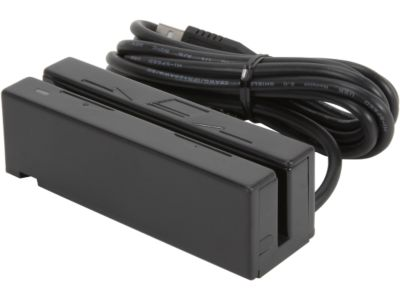
\includegraphics[width=2in]{./media/cardreader.jpg}
        \item Attendance sheets can be manually filled out on the OrgSync website
    \end{itemize}
\end{frame}

\begin{frame}{Event Analytics Opportunity}
    \begin{enumerate}
        \item Student Orgs are starting to collect a lot of data
        \item Org Leaders want to use this data to see if events are succeeding
        \item OrgSync doesn't provide useful tools in this area
    \end{enumerate}
\end{frame}    


\section{Data}

\begin{frame}{Data-Providing Organization}
    The Georgia Tech Catholic Student Organization (GTCSO) was interested in the development of this tool,
    and allowed me to use their data as I built this project. 

    They closely model my target user group:
    \begin{itemize}
        \item The GTCSO hosts 3+ events a week
        \item The GTCSO leadership board does not directly run most of these events,
            but wants to keep track of successes and failures
        \item The GTCSO has several recurring event series, and individual recurrences
            can be meaningfully compared
    \end{itemize}
\end{frame}

\begin{frame}{Dataset Size}
    \begin{itemize}
        \item 24 events
        \item 166 students
        \item 483 attendance records
    \end{itemize}

    % Not nearly what I hoped to reach: The GTCSO had difficulty rolling out 
    % BuzzCard readers to certain types of events, so this data represents a 
    % partial record.

    % \textbf{My focus is on analytics for a single org.} Despite this problem, the GTCSO
    % still provided a larger data set than I could find elsewhere at GT.
\end{frame}

\section{Implementation}

\begin{frame}{Design}
    \begin{itemize}
        \item Developed as a report generation tool
        \item Aimed for high modularity
        \item Implemented a smaller number of more flexible commands
    \end{itemize}
\end{frame}

\begin{frame}{Technologies}
    \begin{itemize}
        \item SQLite for local data store
        \item Python3 for all modules
        \item LaTeX, Pandas, and matplotlib for displaying data
    \end{itemize}
\end{frame}

\begin{frame}{Architecture}
    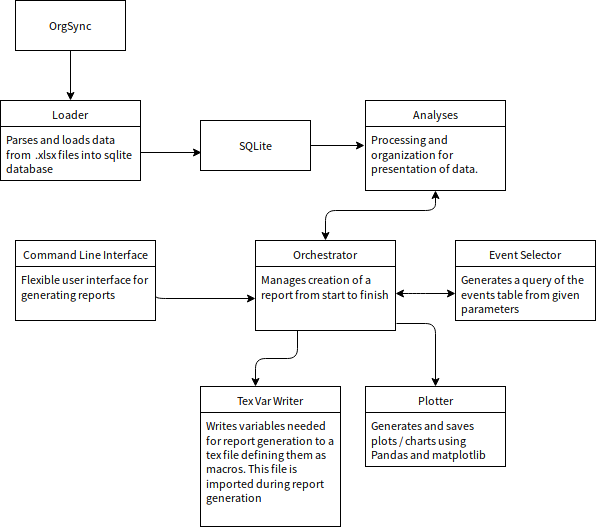
\includegraphics[width=3.8in]{./media/architecture.png}
\end{frame}


\begin{frame}[standout]
    Live Demo
\end{frame}


\section{Future Work}

\begin{frame}{Unimplemented Proposed Features}
    \begin{itemize}
        \item Analytics based on the attendance trends of individuals, in order to identify:
            \begin{itemize}
                \item Events with loyal attendees (somewhat shown through the ``average events attended'' metric)
                \item Events that get attendees to start attending the org's events more frequently afterward
            \end{itemize}
        \item GUI
    \end{itemize}
\end{frame}

\begin{frame}{Other Potential Features}
    \begin{itemize}
        \item Non-OrgSync RFID system for easier data collection. (Faster and semi-anonymous)
        \item Email list generation
        \item Misc. Improvements
            \begin{itemize}
                \item Improved portability
                \item More attractive reports
                \item Fully automated backend
            \end{itemize}
        \item Hosted instance with web interface
        \item Features responding to user feedback 
    \end{itemize}
\end{frame}

\begin{frame}[standout]
    Questions?
\end{frame}


\end{document}
